\section[OpenStack Test Environment \texorpdfstring{{\textbf{\tiny \enspace (JE, SK, NK)}}}{}]{OpenStack Test Environment}
\sectionmark{OpenStack Test Environment}
\label{environment}
As described in Chapter~\ref{related}, we tried various possibilities to install an OpenStack system on a virtual environment. In this chapter we outline the challenges we faced with these possibilities, ultimately leading to the decision to create our own installation routine for a virtual OpenStack environment. Also, we will describe this test environment in detail.\\

\subsection{Existing OpenStack Installation Possibilities}
\label{installpossibilities}
We first tried installing the cloud computing environment HP Helion community edition. It promises an easy installation routine with little need for configuration. Further, it is possible to install HP Helion as an all-in-one system on virtual machines in addition to deploying it on bare-metal. This is an advantage with respect to our requirement of achieving a virtual test environment for reproducible test results. However, even though HP Helion has its advantages for setting up one's own IaaS system for a real use scenario, we came to the conclusion that it is not suitable for our needs. The installation of HP Helion took around 90 minutes on our hardware, which is not feasible for repeated installations. Further, we found that HP Helion does not survive a reboot of the host or the virtual machines it is running on. Fixing this issue would have required understanding the underlying installation scripts, which would still not have been beneficial in understanding OpenStack itself. Additionally, with our limited knowledge of HP Helion, it would have been a challenge to customize the system to fit our needs. We thus concluded that we would not use HP Helion for analyzing the dependability of OpenStack in line with this masters project.\\

A further option for an OpenStack deployment to work with for dependability testing we considered was DevStack. Due to the nature of the use cases for which DevStack is made, multi-node and high-availability setups are not the main focus, and therefore not documented well enough for us to customize DevStack and use it for dependability analyses. Also, it is not possible to generalize results of dependability analyses run on DevStack to a full OpenStack installation, as DevStack is not designed with real deployment in mind. As a result, we decided to use a full OpenStack installation for running our analyses.\\

\subsection{Specifying our own OpenStack Environment}
In order to be able to make the OpenStack test environment installation as easy and quick as possible, so that one can concentrate on the dependability analysis, we chose to install OpenStack virtually. A further advantage of this virtual installation is the reproducibility of experiment results, which is important to be able to make scientific statements about the dependability of OpenStack. We used libvirt\footnote{\url{http://libvirt.org/}} to create a number of virtual machines based on simple configuration files and Ansible\footnote{\url{http://www.ansible.com}} to orchestrate the installation of OpenStack on these nodes. The details of this automated installation are described in Chapter~\ref{installing}.\\

In order to create an useful test environment for dependability experiments, it was necessary to define an architecture. We chose this architecture to be a simplified OpenStack instance, meaning that we focus only the most important of the OpenStack services available. This can be seen as a bottom-up approach, as we focus on evaluating a simpler system than one might encounter when looking at an OpenStack system in production mode. One advantage of this approach is that, due to the simplicity, it is easier to make statements about OpenStack in general, than on one specific system. Libvirt and Ansible allow to add more nodes, create a more complex OpenStack system and, extend the proposed architecture by means of high availability mechanisms. We then draw conclusions about their effectiveness.\\

Figure~\ref{fig:arch} shows our virtual test environment architecture, which is the proposed architecture of the official OpenStack install guide\footnote{\url{http://docs.openstack.org/kilo/install-guide/install/apt/content/index.html}}. All nodes are virtual machines running on a physical host. The tenant virtual machines are dispatched on the compute node by means of nested virtualization. By default, our environment contains the following nodes:
\begin{itemize}
	\item One controller node: this node runs the OpenStack Dashboard (Horizon), the API services, the MySQL database, the RabbitMQ message queue server, the scheduler for the compute resources, Identity (Keystone) and Image (Glance) services.
	\item One network (Neutron) node: this node handles the internal and external routing and DHCP services for the virtual networks.
	\item Two compute nodes: the compute nodes are the computing resources for running the virtual machines of the OpenStack users. They run the hypervisor and services like \verb|nova-compute|, which is responsible for creating and terminating virtual machine instances through the hypervisor APIs.
	\item Two object storage (Swift) nodes: these nodes operate the OpenStack container and object services and each contain two local block storage disks for persisting the objects.
\end{itemize}

Further, the following networks are used to communicate between nodes and instances:
\begin{itemize}
	\item Management network: this network is used for the OpenStack administration, i.e., it connects the OpenStack services on the different nodes. 
	\item Tenant or tunnel network: these networks can be created by the OpenStack users to achieve communication between projects or instances. 
	\item External network: this network provides internet access to the instances.
\end{itemize}

This architecture is comprehensive enough to test various OpenStack use cases and analyze the dependability of the system.\\

\begin{figure}[h]
	\centering
		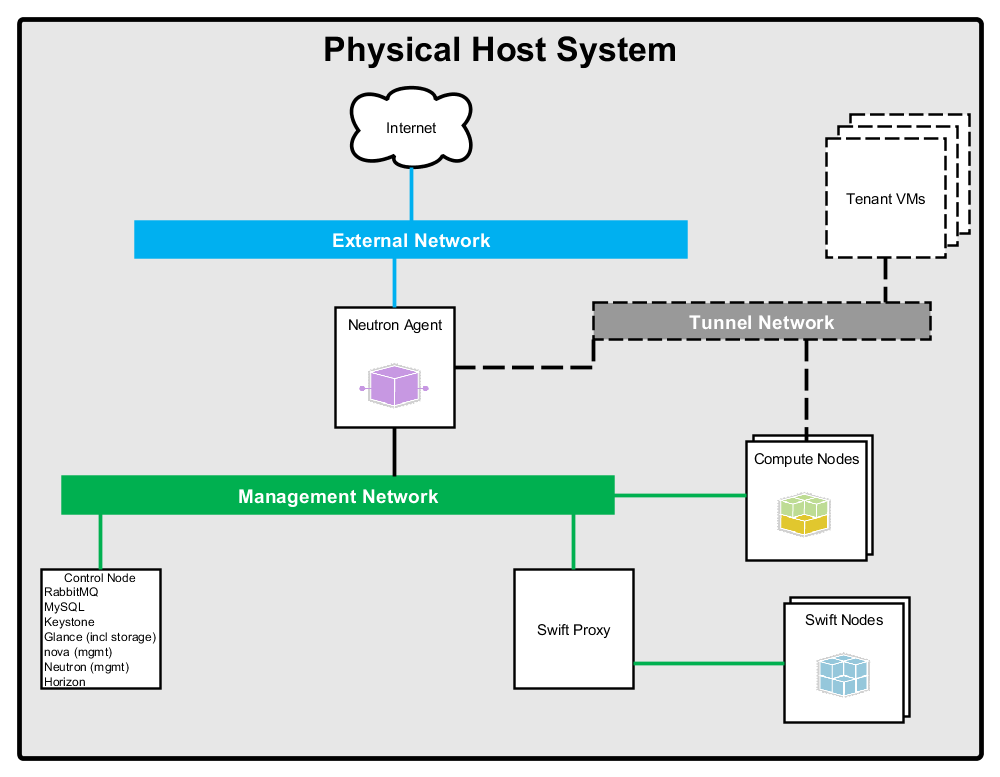
\includegraphics[width=0.90\textwidth]{images/architectureEN.PNG}
	\caption{Our test environment architecture}
	\label{fig:arch}
\end{figure}

The virtual OpenStack installation requires far less hardware resources than a distributed bare metal installation. It is possible to install a fully functional simplified test environment with one compute and object storage node on a quad-core Intel Xeon machine with 8GB RAM. For the full installation, more resources are recommended. We used a 16-core machine with 64GB RAM. 












